\documentclass[10pt]{beamer}
%math
\usepackage{amsmath}
\usepackage{amssymb}
\usepackage{mathtools}
%logic
\usepackage{pgffor}
\usepackage{ifthen}
%science
\usepackage{siunitx}
\usepackage[version=4]{mhchem}
%language
\usepackage[english]{babel}
%formatting
\usepackage{parskip}
%images and plots
\usepackage{graphicx}
\usepackage[justification=centering]{caption}
\usepackage{subcaption}
\usepackage{float}
\usepackage{pgf}
\usepackage{import}
\usepackage{jsonparse}
%tables
\usepackage{booktabs}
\usepackage{makecell}
%citation, quatation and lists
\usepackage{hyperref}
\usepackage[style=numeric,maxcitenames=2,sorting=nty,doi=false,
url=false,isbn=false,eprint=false,note=false,giveninits=true]{biblatex}
\usepackage[noabbrev,nameinlink]{cleveref}
\usepackage{csquotes}
\usepackage{acro}


%setup plugins
\addbibresource{literature.bib}
\def\pgfsysdriver{pgfsys-dvipdfm.def}
\usefonttheme{serif}

\hypersetup{colorlinks=true,linkcolor=blue}
\captionsetup{justification=centering}

\DeclareSIUnit\angstrom{\text {Å}}
\DeclareSIUnit\bar{bar}
\sisetup{range-phrase = { to }}

\usetheme{default}
\setbeameroption{show notes on second screen=right}

\title{A Small Signal MOSFET Model}
\subtitle{Derivation, Application and Generalization}
\author{Simon Legtenborg, 3773994}
\date{September 16, 2025}

\makeatletter
\newcommand{\printfontsize}{\f@size pt}
\makeatother

% Document
\begin{document}

    \begin{frame}
        \titlepage
    \end{frame}
    \note[itemize]{
        \item Welcome to this presentation
        \item Talk roughly 10 minutes about small signal model, cover derivation, 
        application and generalization
    }

    \section{Introduction}
\begin{frame}{Introduction}
	\begin{itemize}
		\item Linear electrical systems are well researched.
		\item Analytical solutions can be found.
		\item Problems in circuit theory arise if nonlinear elements are part of the circuit.
		\item It is only natural to find a linear approximation for circuits to utilize the standard
		tool-set for circuit analysis.
		\item The approximation is only valid in a small interval; only small signals can be 
		analyzed.
	\end{itemize}
\end{frame}
\begin{frame}{Introduction}
	\begin{figure}
		\centering
		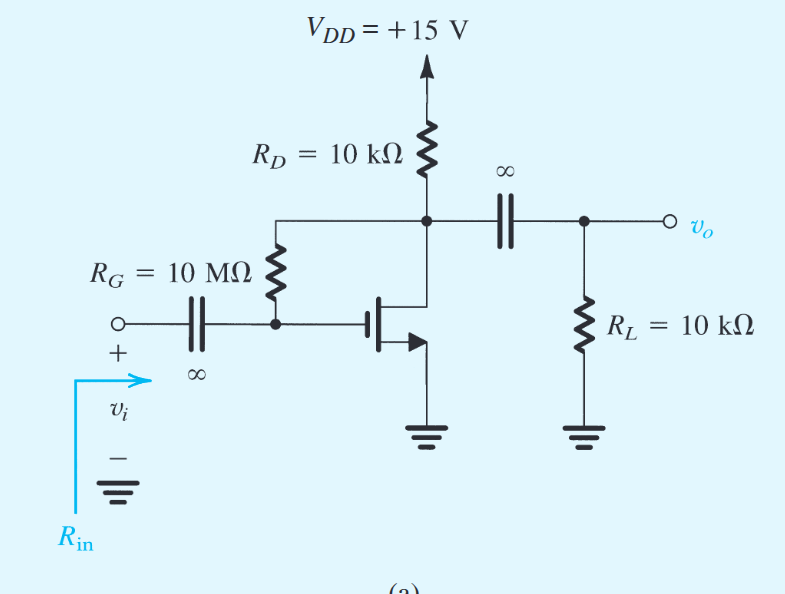
\includegraphics[width=0.7\textwidth]{../assets/example_circuit.png}
		\caption{Example circuit suitable for small signal analysis.}
		\label{fig:example_circuit}
	\end{figure}
\end{frame}

    \note[itemize]
        {
            \item MOSFET is the simplest model.
            \item It is the most researched.
            \item It serves as the best introductory example for short presentation
            \item Zoom in for application.
            \item Small signal model is only useful if one knows small signal analysis.
            \item Zoom out for the greater picture.
        }

    \section{Derivation of a MOSFET Small Signal Model}
\begin{frame}{Derivation: Notational Conventions}
    \begin{itemize}
        \item DC quantities are labeled with UPPERCASE variables and UPPERCASE subindices: 
        $V_{\mathrm{GS}}$
        \item Pure AC quantities are labeled with lowercase variables and lowercase subindices: 
        $v_{\mathrm{gs}}$
        \item Superpositions of both quantities are labeled with lowercase variables and 
        UPPERCASE subindices: $v_{\mathrm{GS}}=V_{\mathrm{GS}}+v_{\mathrm{gs}}$

        \begin{figure}
            \centering
            \includegraphics{../plots/notational_convention.pdf}
            \caption{Notational conventions for DC and AC quantities.}
            \label{fig:signal_convention}
        \end{figure}
    \end{itemize}
\end{frame}

\begin{frame}{Derivation: MOSFET Current-Voltage Characteristics}
    \vspace{0.5cm}
    \begin{figure}
        \centering
        \includegraphics{../plots/cv_characteristics.pdf}
        \caption{MOSFET current-voltage characteristics.}
        \label{fig:mosfet_characteristics}
    \end{figure}
    \begin{itemize}
        \item Require saturation-region operation: $V_{\mathrm{DS}}\gg V_{\mathrm{GS}}-V_{\mathrm{t}}$
        \item In this regime, the following current-voltage characteristics are valid:
            \begin{itemize}
                \item $i_{\mathrm{drain}}=\frac{1}{2}k_{\mathrm{n}}(v_{\mathrm{gate}}-V_{\mathrm{t}})^{2}$
                \item $i_{\mathrm{gate}}=0$
            \end{itemize}
    \end{itemize}
\end{frame}

\begin{frame}{Derivation: Signal Current in Drain Terminal}
    \begin{itemize}
        \item Apply a signal $v_{\mathrm{GS}}=V_{\mathrm{GS}}+v_{\mathrm{gs}}$ to the gate terminal.
        \item This results in the following drain current:
    \end{itemize}
    \begin{block}{}
        \setlength{\abovedisplayskip}{0pt}
        \setlength{\belowdisplayskip}{0pt}
        \begin{align*}
            i_{\mathrm{D}}&=\frac{1}{2}k_{\mathrm{n}}(V_{\mathrm{GS}}+v_{\mathrm{gs}}
            -V_{\mathrm{t}})^{2} \\
            &=\underbrace{ \frac{1}{2}k_{\mathrm{n}}(V_{\mathrm{GS}}-V_{\mathrm{t}})^{2} }_{ =I_{\mathrm{D}}}+
            k_{\mathrm{n}}(V_{\mathrm{GS}}-V_{\mathrm{t}})v_{\mathrm{gs}}
            +\frac{1}{2}k_{\mathrm{n}}v_{\mathrm{gs}}^{2}
        \end{align*}
    \end{block}
    \begin{itemize}
        \item The third term is negligible for sufficiently small $v_{\mathrm{gs}}$, i.e. 
        $v_{\mathrm{gs}}\ll 2(V_{\mathrm{GS}}-V_{\mathrm{t}})$.

    \end{itemize}
\end{frame}

\begin{frame}{Derivation: Signal Current in Drain Terminal}
    \begin{block}{}
        \begin{itemize}
            \item Neglecting the third term under the specified condition results in the following 
            expression for the drain current $i_{\mathrm{D}}$:
        \end{itemize}
        \begin{align*}
                i_{\mathrm{D}}&=I_{\mathrm{D}}+i_{\mathrm{d}} \\
                I_{\mathrm{D}}&=\frac{1}{2}k_{\mathrm{n}}(V_{\mathrm{GS}}-V_{\mathrm{t}})^{2} \\
                i_{\mathrm{d}}&=k_{\mathrm{n}}(V_{\mathrm{GS}}-V_{\mathrm{t}})v_{\mathrm{gs}}
        \end{align*}
    \end{block}

    \begin{itemize}
        \item the parameter, that related $i_{\mathrm{d}}$ and $v_{\mathrm{gs}}$ is called the 
        transconductance $g_{\mathrm{m}}=k_{\mathrm{n}}(V_{\mathrm{GS}}-V_{\mathrm{t}})$ 
    \end{itemize} 
\end{frame}

\begin{frame}{Derivation: Linear Circuit}
    \begin{itemize}
        \item A linear circuit is a circuit that obeys the superposition principle:
        \begin{itemize}
            \item Let the output of the circuit be $F(x)$.
            \item Let the input signal be a linear combination $a x_{1}(t)+b x_{2}(t)$.
            \item The circuit satisfies $F(a x_{1}(t) + b x_{2}(t)) = a F(x_{1}(t)) + b F(x_{2}(t))$.
        \end{itemize}
        \item Circuits made of ideal resistors, capacitors, inductors, voltage- and current sources are linear circuits.
        \item Circuits are nonlinear if they have nonlinear components (e.g., diodes, transistors).
        \item When small signals are applied, transistors tend to behave approximately linearly:
        \begin{itemize}
            \item They can be replaced with a small signal model.
            \item This allows the use of linear analysis techniques.
        \end{itemize}
    \end{itemize}
    \note[item]{Other components, whole digital logic circuits}
\end{frame}

\begin{frame}{Deviation: Small-Signal Equivalent Circuit}
    \begin{itemize}
        \item Signal analysis can be simplified by separating DC calculation from small-signal calculation.
        \item Only care about the signal components and assume one steady bias point.
        \item From the preceding analysis, we get the following equations.
        \begin{itemize}
            \item $i_{\mathrm{g}}(v_{\mathrm{gs}}, v_{\mathrm{ds}})=0$ \\
            \item $i_{\mathrm{d}}(v_{\mathrm{gs}}, v_{\mathrm{ds}})=g_{\mathrm{m}}v_{\mathrm{gs}}$
        \end{itemize}
        \item A circuit that satisfies these equations is called a small-signal equivalent circuit.
    \end{itemize}
\end{frame}

\begin{frame}{Deviation: Small-Signal Equivalent Circuit}
    \begin{figure}
        \centering
        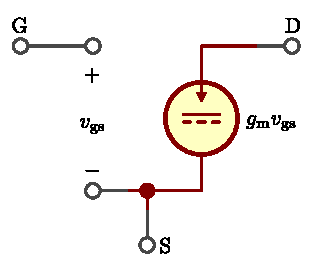
\includegraphics{../assets/small_signal.pdf}
        \caption{Small-signal equivalent circuit of a MOSFET.}
        \label{fig:mosfet_small_signal_model}
    \end{figure}
\end{frame}
    \section{Application in Circuit Analysis}

\begin{frame}{Application: MOSFET Amplifier}
    \begin{figure}
        \centering
        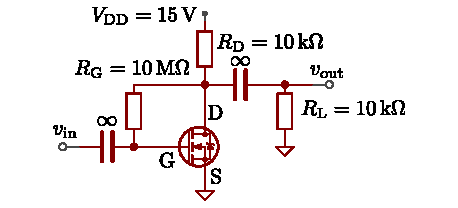
\includegraphics{../assets/example_circuit_small.pdf}
        \caption{MOSFET amplifier circuit.}
        \label{fig:mosfet_amplifier}
    \end{figure}

    What is the amplification $v_\mathrm{out}/v_\mathrm{in}$ of this amplification circuit?
    \begin{enumerate}
        \item Identify DC operating point.
        \item Replace MOSFET with small signal model.
        \item Analyze resulting linear circuit.
    \end{enumerate}
\end{frame}

\begin{frame}{Application: DC Operating Point}
    \begin{itemize}
        \item Replace AC sources with short circuits
        \item large capacitors act as open circuits for DC signals
    \end{itemize}
    \begin{figure}
        \centering
        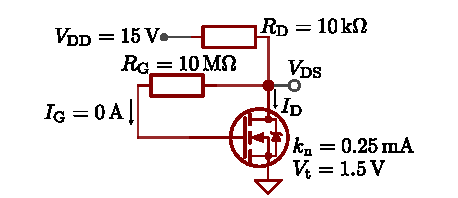
\includegraphics{../assets/example_circuit_dc.pdf}
        \caption{Reduced amplifier circuit, DC operating point.}
        \label{fig:mosfet_amplifier_dc}
    \end{figure}
    \begin{align*}
        I_{\mathrm{D}}&=\frac{1}{2}k_{\mathrm{n}}(V_{\mathrm{GS}}-V_{\mathrm{T}})^{2} 
        = \qty{1.06}{\milli \ampere}\\
        V_{\mathrm{GS}}&=V_{\mathrm{DS}}=V_{\mathrm{DD}}-R_{\mathrm{D}}I_{\mathrm{D}}
        =\qty{4.4}{\volt} \\
        g_\mathrm{m} &= k_\mathrm{n} (V_\mathrm{GS}-V_t) = \qty{0.725}{\milli \ampere \per \volt}
    \end{align*}
\end{frame}

\begin{frame}{Application: Small Signal Replacement}
    \begin{itemize}
        \item Replace DC sources with short circuits
        \item large capacitors act as short circuits for high frequency signals
        \item Simplify circuit using linear circuit analysis
    \end{itemize}
    \begin{figure}
        \centering
        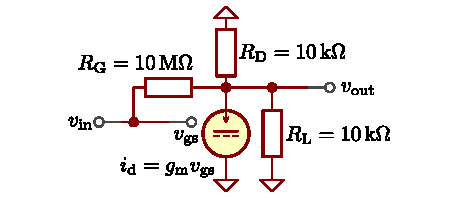
\includegraphics{../assets/mosfet_amplifier_small_signal.pdf}
        \caption{Reduced amplifier circuit, small signal model.}
        \label{fig:mosfet_amplifier_ac}
    \end{figure}
\end{frame}

\begin{frame}{Application: Small Signal Analysis}
    \begin{itemize}
        \item Simplify circuit by combining both resistors
    \end{itemize}
    \begin{figure}
        \centering
        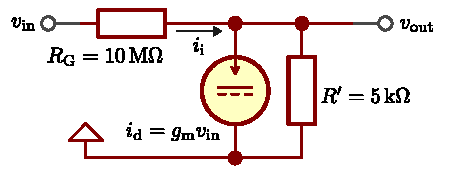
\includegraphics{../assets/mosfet_amplifier_small_signal_reduced.pdf}
        \caption{Reduced amplifier circuit, small signal model.}
        \label{fig:mosfet_amplifier_ac_2}
    \end{figure}

    \begin{align*}
        R'=R_\mathrm{D} \parallel R_\mathrm{L} &= \qty{5000}{\ohm} \\
        v_{\mathrm{in}}-v_{\mathrm{out}}&=R_{\mathrm{G}} i_{\mathrm{i}} \\
        (g_{\mathrm{m}}v_{\mathrm{gs}})+v_{\mathrm{out}} /R'&=i_{\mathrm{i}}
    \end{align*}
\end{frame}

\begin{frame}{Application: Small Signal Analysis}
    \begin{figure}
        \centering
        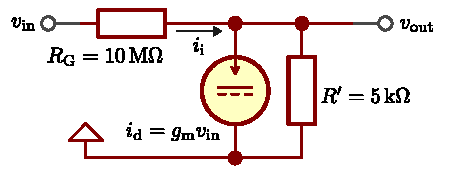
\includegraphics{../assets/mosfet_amplifier_small_signal_reduced.pdf}
        \caption{Reduced amplifier circuit, reduced small signal model.}
        \label{fig:mosfet_amplifier_ac_reduced}
    \end{figure}
    \begin{itemize}
        \item Solve for the amplification:
    \end{itemize}
    \begin{align*}
        v_{\mathrm{in}}-v_{\mathrm{out}}&=R_{\mathrm{G}}\left( g_{\mathrm{m}}v_{\mathrm{in}}+\frac{v_{\mathrm{out}}}{R'} \right) \\
        v_{\mathrm{out}}\left( -1-\frac{R_{\mathrm{G}}}{R'} \right)&=v_{\mathrm{in}}(-1+R_{\mathrm{G}}g_{\mathrm{m}}) \\
        \frac{v_{\mathrm{out}}}{v_{\mathrm{in}}}&=\frac{1-R_{\mathrm{G}}g_{\mathrm{m}}}{1+R_{\mathrm{g}} / R'}=\num{-3.6}
    \end{align*}
    
\end{frame}
    \section{Generalization}
\begin{frame}{Generalization}
    \begin{itemize}
        \item The procedure for deriving small signal models can be generalized to other 
        transistor types and more complex models
        \item Find large signal models (for low frequency): 
        $i_{\mathrm{drain}}(v_{\mathrm{gate}}, v_{\mathrm{drain}})$ and 
        $i_{\mathrm{gate}}(v_{\mathrm{gate}}, v_{\mathrm{drain}})$
        \item Linearize the large signal models using a Taylor approximation
    \end{itemize}
    \begin{align*}
        i_{\mathrm{drain}}(&V_{\mathrm{GS}}+v_{\mathrm{gs}},
        V_{\mathrm{DS}}+v_{\mathrm{ds}})\simeq i_{\mathrm{drain}}
        (V_{\mathrm{GS}},V_{\mathrm{DS}}) \\
        &+\left.\frac{\partial i_{\mathrm{drain}}}{\partial v_{\mathrm{gate}}}\right|
        _{(V_{\mathrm{GS}},V_{\mathrm{DS}})} v_{\mathrm{gs}} 
        + \left. \frac{\partial i_{\mathrm{drain}}}{\partial v_{\mathrm{drain}}} \right|
        _{(V_{\mathrm{GS}},V_{\mathrm{DS}})} v_{\mathrm{ds}} \\
        i_\mathrm{gate}(&V_{\mathrm{GS}}+v_{\mathrm{gs}},
        V_{\mathrm{DS}}+v_{\mathrm{ds}})\simeq i_{\mathrm{gate}}
        (V_{\mathrm{GS}},V_{\mathrm{DS}}) \\
        &+\left.\frac{\partial i_\mathrm{gate}}{\partial v_{\mathrm{gate}}}\right|
        _{(V_{\mathrm{GS}},V_{\mathrm{DS}})} v_{\mathrm{gs}} 
        + \left. \frac{\partial i_\mathrm{gate}}{\partial v_{\mathrm{drain}}} \right|
        _{(V_{\mathrm{GS}},V_{\mathrm{DS}})} v_{\mathrm{ds}}
    \end{align*}
\end{frame}
\note[itemize]{
    \item High frequency models can be derived by including $\dot{v}_{\mathrm{gate}}$ and 
        $\dot{v}_\mathrm{drain}$ in the current voltage characteristics
    \item Partial derivatives are expression for conductance of transconductance in circuit
    }

    \begin{frame}{References}
        \nocite{*}
        \printbibliography[shortauthor=true]
    \end{frame}

\end{document}
